%%%%%%%%%%%%%%%%%%%%
%                                              %
%                 Error Analysis               %
%                                              %
%%%%%%%%%%%%%%%%%%%%

\labChapter{}{Error Analysis}

In laboratory work, it is usually necessary to use experimental apparatus to measure physical quantities. The measurements are seldom, if ever, perfect. As a result, imperfections must be taken into account in any set of physical measurements. One of the most important things to be learned in the laboratory is how to make reliable estimates of the uncertainties involved in any physical measurements and how to handle the propagation of these errors, i.e., to know how the uncertainties affect calculated results of an experiment.


% Types of Errors
\section{Error Analysis Procedure}
\label{sec:ErrorProc}

This section is a guide to performing error analysis for an experiment.  The steps are detailed in the following sections.
\begin{itemize}
\item[\(\triangleright\)] Identify the likely sources of measurement error.
  \begin{itemize}
  \item Measurement errors can stem from the instrumentation, the experimental setup and procedure.
  \item Explain whether errors are systematic or random (\ref{sec:TypesErrors}).
  \end{itemize}
\item[\(\triangleright\)] Estimate the magnitude of the measurement errors using:
  \begin{itemize}
  \item the specification of the equipment,
  \item significant digits displayed,
  \item your estimate of how accurately you can read the instrument,
  \item the range or standard deviation of repeated measurements (\ref{sec:TypesErrors}).
  \end{itemize}
\item[\(\triangleright\)] Calculate the magnitude of the expected error in calculated experimental quantities due to your measurement errors (\ref{sec:ErrorPropagation}).
\item[\(\triangleright\)] If the difference between your results and expected results is much more than the magnitude of error you expect, look for a cause for the difference, including:
  \begin{itemize}
  \item a problem in how the experiment was performed,
  \item a calculation problem, a units conversion error, or using a trig function with degrees instead of radians,
  \item your estimate of the measurement error is too small,
  \item an error in some common value used in the calculations.
  \end{itemize}
\item[\(\triangleright\)] Report your results with the correct number of significant digits (\ref{sec:SigFig}) and with the calculated error.
\end{itemize}

\section{Types of Errors}
\label{sec:TypesErrors}

Experimental measurements are characterized by accuracy and precision. As illustrated in Fig.~\ref{fig:PreciseAccurate}, a set of measurements is precise and accurate if the average value of many measurements is close a known or expected value. A set of measurements is precise if they are closely clustered around their average value. Random errors cause more scatter in the results and reduce the precision of a measurement. Random measurement errors can be due to the inherent limitations of the equipment. They can be estimated and reduced by repeated measurements.  Systematic or precision errors can be due to equipment calibration or approximations in analysis. They reduce the precision of the experiment and are not reduced by repeated measurements. Often you can estimate precision errors by considering the equipment and its specifications.

\begin{figure}%[htbp] %  figure placement: here, top, bottom, or page
  \begin{center}
    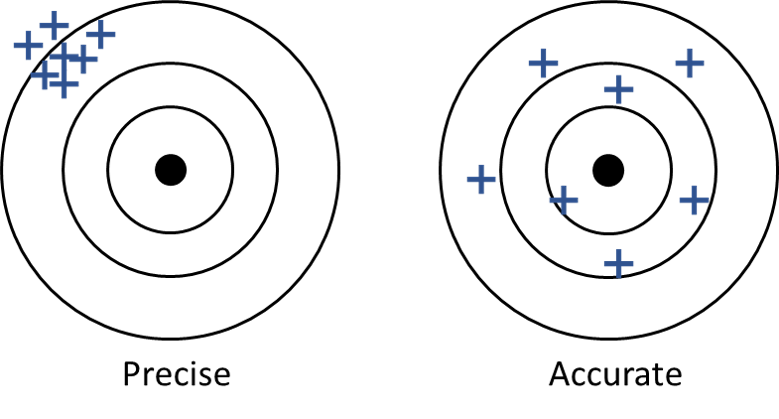
\includegraphics[width=3in]{{IntroductionFigures/ErrorType.png}}
  \end{center}
  \caption{The distinction between precision and accuracy.}
  \label{fig:PreciseAccurate}
\end{figure}

Error analysis can help you recognize if your results are consistent with a known or expected value. Each measurement has some combination of systematic and random errors. Make your best estimate of the possible error in each measured value. Your estimate may include instrument limitations and variation of measurements over multiple trials. Calculate the differences between your experimental results and any known values. Recalculate the experimental value in your spreadsheet by changing your measurements by adding or subtracting the estimated errors. Observe the range of experimental values (maximum and minimum) that you find in these recalculations.  If the expected values fall too far outside this range, there is some problem which you need to address.

Suppose you are measuring the density of a rectangular block. The block has dimensions $L=2.00\,\centi\meter$,  $ W=3.00\,\centi\meter$ and $H=5.00\,\centi\meter$. The mass of the block is $M=60.00\,\gram$. The uncertainty in the length measurements is $\pm0.01\,\centi\meter $ and the uncertainty in the mass is $\pm0.05,\gram$. The calculated density is mass divided by volume. The value calculated directly from your measurements is $\rho_{\mbox{expt}} = \nicefrac{60.00\,\gram}{30.00\,\centi\meter\cubed} = 2.00\,\gram\per\centi\meter\cubed $. The maximum density consistent with your measurements is the ratio of the maximum mass and the minimum volume: \(\rho_{\mbox{max}} = \nicefrac{60.05\,\gram}{\left(1.99\times0.99\times4.99\,\centi\meter\cubed\right)} = 2.02\,\gram\per\centi\meter\cubed\). Similarly, the minimum density consistent with your result is $1.98\,\gram\per\centi\meter\cubed$. If the expected density is not in this range, you need to consider possible explanations: the errors in the measurements could be larger than you estimated, the actual density could be different from the expected value, your calculation may be wrong, or perhaps the shape is not exactly rectangular.

The two types of errors illustrated in Fig.~\ref{fig:PreciseAccurate} require different treatment. The systematic errors illustrated on the target labelled ``Precise'' cannot be reduced by taking more measurements, while the average value obtained with the random errors on the target labelled ``Accurate'' improves with more measurements. The following sections provide guidance on analyzing systematic and random errors.

% Random Errors
\subsection{Random Errors}
\label{sub:RandomErrors}

Random errors are inherent in almost all measurements. They arise because of uncontrollable conditions affecting the observer, the measuring device, and the quantity to be measured. On the basis of probability it is assumed that these errors are as likely to be positive as negative, and more likely to be small than large. Taking a number of independent measurements of a given physical quantity and using the arithmetic average of these values in any computation may therefore minimize their effect. This minimization is only achieved if the measurements are independent. A common mistake is biasing a new measurement to agree with the previous measurements. This mistake makes the measurements more precise, but less accurate as shown in Fig.~\ref{fig:PreciseAccurate}. Taking truly independent measurements is the best way to reduce random error.

%The precision with which a physical quantity has been measured depends upon the spread of the set of measurements about their mean value. If the separate measurements are widely dispersed about the mean, the precision is low.  If the separate measurements are all close, the precision is high. There are many methods of estimating the spread of a set of measurements about the mean value. In general, one usually determines the deviations of the measured values from the mean value and then uses some function of these deviations to represent the spread, and thus the precision of the set of measurements.

The most well established method to quantify the spread of random errors in a measurement is to compute the {\it standard deviation}. Suppose you make $N$ measurements $x_1$, $x_2$, \ldots, $x_N$ of a certain quantity $x$. The average value is
\begin{equation}
  \label{eq:errorMeanX}
  \bar{x}=\frac{x_1 + x_2 + \ldots + x_N}{N}=\frac{1}{N}\sum_{i=1}^N x_{i},
\end{equation}
and the standard deviation of the individual measurements is
\begin{equation}
  \label{eq:errorSigmaX}
  \sigma = \sqrt{\frac{(x_1-\bar{x})^2 + (x_2-\bar{x})^2 + \ldots + (x_N-\bar{x})^2}{N-1}} = \sqrt{\frac{1}{N-1} \sum_{i=1}^{n}\left(x_i-\bar{x}\right)^2}.
\end{equation}
In Excel these operations can be carried out using the functions \texttt{AVERAGE()} and \texttt{STDEV()} or \texttt{STDEV.S()}.

If you perform many measurements, then your estimate of the average value improves. The ``standard deviation of the mean'' for $N$ measurements is
\begin{equation}
  \label{eq:errorSigmaMeanX}
  \sigma_{\mbox{mean}} = \frac{\sigma}{\sqrt{N-1}}.
\end{equation}
Your best estimate of a measurement $x$ is then $\bar{x} \pm \sigma_{\mbox{mean}}$.

For example, suppose that four measurements of a length yield, in centimeters, 7.65, 7.61, 7.66, 7.68.  The mean value is
\[
\bar{x} = \left(7.65 + 7.61 + 7.66 + 7.68\right)/4\,\centi\meter
        = 7.65\,\centi\meter,
\]
and the standard deviation is
\[
\sigma = \sqrt{\frac{(7.65-7.65)^2 + (7.61-7.65)^2 + 
                     (7.66-7.65)^2 + (7.68-7.65)^2}{4-1}\centi\meter\squared}
       = 0.029\,\centi\meter.
\]
The standard deviation of the average value is thus reduced to $ 0.029\,\centi\meter / \sqrt{3} =  0.017\,\centi\meter $ and therefore the best estimate of the length is $\bar{x} =  7.65\,\centi\meter \pm 0.017\,\centi\meter$.

%A simple but effective measure of the spread of indeterminate errors in the measurement of a quantity is the average deviation from the mean. Thus, if a given quantity is measured several times and the mean value of these measurements is computed, then the indeterminate error may be represented by the average difference between the mean value and the measured values without regard to sign. For example, suppose that four measurements of a length yield, in centimeters, 7.65, 7.61, 7.66, 7.68. The mean value is 7.65. The deviations without regard to sign are 0.00, 0.04, 0.01, 0.03. The average deviation from the mean is 0.02. If this average deviation is first subtracted from, and then added to, the mean value, an interval is defined (7.63 to 7.67), which generally brackets about half of the measured values. In this example the measurements 7.65 and 7.66 lie within the interval but 7.61 and 7.68 lie outside the interval. In many cases, it is desirable to extend the interval so as to include almost all the measured values, which can generally be done by using twice the average deviation as a measure of the indeterminate errors. The interval in the above example then becomes $7.65 \pm 0.04$ and includes all the measured values.

Frequently, a set of measurements has to be taken in an experiment under a prescribed condition. It may be difficult to judge exactly when this condition is satisfied. In this case, it may be necessary to vary the physical quantities that produce this condition and to note how much each may be varied without appreciably altering the prescribed condition. This variation may be used to determine the error.

Finally, the measuring devices (meter stick, voltmeter, and so on) are not perfectly accurate even if one could make a precise reading with them. The manufacturer specifies the accuracy in the measuring device; for example, a particular type of voltmeter may be guaranteed to give readings accurate to $\pm 1\%$ of full scale reading. Part of this tolerance is random error that can average out by taking multiple readings. As discussed in the next section, another part of the instrument error is systematic. An ammeter may always read $0.5\%$ high because of the value of a resistor internal to the device.

% Systematic Errors
\subsection{Systematic Errors}
\label{sub:SystematicErrors}

Systematic errors occur in an experiment because of a defective measuring apparatus, faulty methods, or incomplete working equations. They are definite in sign and magnitude and cannot be reduced by taking the average of a number of measurements, because the same error is included in each measurement.
These errors are often more important than the random errors. Calibrating the measuring apparatus, modifying the method, or changing the working equations may reduce them. These procedures are generally described as corrections that are to be made in performing the experiment.
For example, the reading of a Vernier caliper may not be zero when the jaws are in contact. This so-called zero error must be corrected for in using the instrument, i.e., the instrument must be calibrated. Otherwise, all measurements made with the caliper will be in error by a determinate amount, the zero error.

In many experiments time is measured with a stopwatch. Using a stopwatch that does not run at the proper rate would introduce an instrumental systematic error. A watch that ran too fast would cause all times recorded to be too high. A more significant systematic error encountered with a stopwatch is reaction time error. In measuring the time for an air track glider to travel down an incline, the observer may introduce a systematic error due to the reaction time required to stop the watch and a random error due to variation in reaction time. Report this source of error as ``reaction time error.'' The expression ``human error'' is too ambiguous to be useful in describing measurement errors.

%An example of personal systematic error is the tendency to look favorably at the first reading taken and then with suspicion on subsequent readings that differ. Other personal errors can be attributed to eyestrain, fatigue, or the position of the eye relative to a scale. Sloppy alignment of the end of a meterstick or failure to properly zero a balance are personal systematic errors which can be avoided with due diligence.

\subsection{Difference between Experimental Value and Expected Value}
\label{sub:ExperimentExpected}

If the true value of a quantity is known, then the systematic error can be estimated as difference between the result observed (experimental value) and the expected value. It is important to remember that this is an estimate of the systematic error. The difference between your experimental value and the expected value is \textbf{not an estimate of the random experimental error}. To report this difference as a percentage, divide the difference by the true value and multiply by 100\%. In Excel, use percent format instead of multiplying by 100\%.

%\begin{align} %
%        \%-\mbox{difference} = \frac{\mbox{Experimental Value} - \mbox{Actual Value}}{\mbox{Actual Value}} \, 100 \%
%\end{align}

If the true value of a quantity is known, then the difference between the experimental value and the expected value must be compared with the estimated systematic and random errors.  The difference between your experimental value and the expected value is \textbf{not an estimate of the experimental error}. To report this difference as a percentage, divide the difference by the true value and multiply by 100. In Excel, use percent format instead of multiplying by 100.

The percent difference between the experimental value and the expected value is
\[
\frac{\mbox{Experimental Value} - \mbox{Actual Value}}{\mbox{Actual Value}} \times 100\%.
\]
For example, suppose a student measures the value of gravity and finds it to be $9.41\,\meter\per\second\squared$, while the standard value is $9.803\,\meter\per\second\squared$.
The systematic relative difference, expressed as a percentage, is $\nicefrac{-0.39}{9.803} \times 100\% = -4.1\%$.
%The difference is $- 0.40 \meter\per\second\squared$.  It is important to maintain the proper sign of the error.
There is no definite allowable difference between the experimental and expected values in the following experiments. However, all measurements should be made with the greatest care, so as to reduce the error as much as possible.

It should be noted that the percent difference is not an estimate of experimental error. Any measurement has random and systematic errors even if the percent difference happens to be small.  Often, scientists do not know the actual value of the quantity they are measuring and they give their best estimate with error. Comparing the difference of the experimental value and the actual value with your best estimate of the experimental error will help determine if there is a systematic error in your results. If the difference is less than your estimated random error, then the results are consistent with the expected value. Having a zero percent difference could be the result of a lucky cancellation of errors and still just means the results are consistent. If the difference is significantly more than the estimated error, then you can begin to ask why your result is not consistent with the expected value.

% Propagation of Systematic Errors
\section{Propagation of Errors}
\label{sec:ErrorPropagation}

Through indirect measurement, the effect of systematic errors can be followed through the equations used. Two simple examples will be discussed.

% Calculation from a single, direct measurement
\subsection{Calculation from a Single, Direct Measurement}

Consider the volume of a sphere $V$ as calculated from a direct measurement of its diameter, $D$.  We would use
\[
  V = \frac{1}{6} \pi \, D^3
\]
where $\pi = 3.1415926\ldots$.  Suppose the value of $D$ is measured as $3.04\,\centi\meter$ and $V$ computed to be $14.71\,\centi\meter\cubed$. It is later discovered that the value of $D$ has a systematic error $\Delta D = +0.01\,\centi\meter$, (unnecessarily large, in all probability). What is the error $\Delta V$ in $V$ and the correct value of $V$?

\begin{enumerate}
\item Direct, brute-force method:\\
  Correct $D$ to $3.03\,\centi\meter$; re-compute $V_{\mbox{corr}}$ as $14.56\,\centi\meter\cubed$.\\
  The systematic error $\Delta V$ in $V$ is then $V - V_{\mbox{corr}} = 0.15\,\centi\meter\cubed$ or +1\%
\item Method based on calculus:\\
  Find the derivative of $V$ with respect to $D$,
  \begin{equation}
    \label{Eq:errorCalcMethod}
    \begin{aligned} %
      \frac{{\rm d}V}{{\rm d}D} &= \frac{3}{6} \pi D^2\\
           {\rm d}V             &= \frac{3}{6} \pi D^2 {\rm d}D.
    \end{aligned}
  \end{equation}
  Note that this shows a direct dependence of a change in $V$ on an infinitesimal change in $D$. Now divide through by $V = \frac{1}{6} \pi \, D^3$
  \[
    \frac{{\rm d}\,V}{V} = 3 \, \frac{{\rm d}\, D}{D}.
  \]
  If a finite change in $D$, such as the systematic error $\Delta D$, is small compared to $D$, then ${\rm d}\,V$ and ${\rm d}\,D$ can be approximated by $\Delta V$ and $\Delta D$, respectively, and so the following can be written:
  \[
    \frac{\Delta V}{V} \approx 3 \, \frac{\Delta D}{D}.
  \]
  This means that the fractional or percent error in $V$ is very nearly 3 times as large as that in $D$. Therefore,
  \[
    \frac{\Delta V}{V} \approx + 3 \, \frac{0.01}{3.04} \approx 1 \%.
  \]
  Hence,
  \[
    \Delta V \approx 0.15\,\centi\meter\cubed
  \]
  and
  \[
    V_{\mbox{corr}} = V - \Delta V = 14.56\,\centi\meter\cubed.
  \]
\end{enumerate}

\subsection{Calculation from Two or More Direct Measurements}

Consider the volume $V$ of a right, circular cylinder as calculated from its diameter $D$ and length $L$. For convenience, let $D$ be measured as $2.00\,\centi\meter$  and $L$ as $5.00\,\centi\meter$. Then,
\[
  V = \frac{1}{4} \pi \, L \, D^2 = 15.71\,\centi\meter\cubed.
\]
If $D$ has an error of $+0.01\,\centi\meter$ and $L$ an error of $-0.02\,\centi\meter$, what is the error $\Delta V$ in $V$ and what is the correct value of $V$?
\begin{enumerate}
\item Direct, brute-force method:\\
  To obtain $V_{\mbox{corr}}$, subtract $0.01\,\centi\meter$ from $D = 2.00\,\centi\meter$, add $0.02\,\centi\meter$ to $L = 5.00\,\centi\meter$ and recompute $V_{\mbox{corr}}$ as $15.61\,\centi\meter\cubed$, whereby $\Delta V$ must be $+0.01\,\centi\meter\cubed$.

\item Method based on calculus:\\
  Find the partial derivatives of $V$
  \[
    \frac{\partial V}{\partial L} =\frac{1}{4} \pi \, D^2   \hspace{2 cm}   \frac{\partial V}{\partial d} =\frac{1}{2} \pi \, D \, L
  \]
  \[
    {\rm d}\, V = \frac{\partial V}{\partial L} \, {\rm d}\, L + \frac{\partial V}{\partial D} \, {\rm d}\, D
  \]
  so that
  \[
    \Delta V \approx \frac{\partial V}{\partial L} \, \Delta L + \frac{\partial V}{\partial D} \, \Delta D = \frac{\pi}{4} \, D^2 \, \Delta L + \frac{\pi}{2} \, D \, L \, \Delta D.
  \]
  Now dividing through by $V = \frac{1}{4}\pi \, D^2 \, L$
  \[
    \frac{\Delta V}{V} \approx \frac{\Delta L}{L} + \frac{2 \Delta D}{D}.
  \]
  i.e.\ the fractional (or percent) systematic error in $V$ is very nearly equal to the fractional systematic error in $L$ plus twice the fractional error in $D$.  In our case,
  \[
    \frac{\Delta L}{L} = \frac{-0.02}{5.00} = -0.4 \%
  \]
  and
  \[
    \frac{2\Delta D}{D} = \frac{+0.02}{2.00} = +1.0 \%
  \]
  so that
  \[
    \frac{\Delta V}{V} \approx +0.6 \%.
  \]

  Thus $\Delta V = +0.09\,\centi\meter\cubed $, i.e.\ the systematic error, is  $+0.09\,\centi\meter\cubed$, the correction is $-0.09\,\centi\meter\cubed$ and $V_{\mbox{corr}} = +15.62\,\centi\meter\cubed $.
\end{enumerate}
% Significant Figures

\section{Significant Figures}
\label{sec:SigFig}

The number of digits required to express the result of an experimental measurement, so that it reflects the accuracy with which the measurement was made, are known as significant figures. Thus, the number of significant figures reflects the limitation of the measuring device and/or the experimenter. Whether the calculations are performed by hand or on a computer, the number of significant figures displayed in the final result must reflect the limitations of the experimental measurement. Often, a computer program will, by default, display either too many or too few digits. If too few digits are displayed, you need to adjust the program setting to show more digits.

For example, if the length of a cylinder is measured as $20.64\,\centi\meter$, this quantity is said to be measured to four significant figures.  If written as  $0.0002064\,\kilo\meter$, we still have only four significant figures. The zeros preceding the ``2'' are used only to indicate the position of the decimal point. The zero between the ``2'' and the ``6'' is a significant figure, but the other zeros are not.  If the above measurement is made with a meter stick, the last digit recorded is an estimated figure representing a fractional part of a millimeter division. All recorded data should include the last estimated figure in the result, even though it may be zero. If this measurement had appeared to be exactly $20$, it should have been recorded as $20.00\,\centi\meter$, since lengths can be estimated by means of this instrument, to about $0.01\,\centi\meter$. When the measurement is written as $20\,\centi\meter$ it indicates that the value is known to be somewhere between $19.5\,\centi\meter$ and $20.5\,\centi\meter$, whereas the value is actually known to be between $19.995\,\centi\meter$ and $20.005\,\centi\meter$.  Conversely, retaining too many significant figures implies greater accuracy than the figures actually represent.

When deciding the number of significant figures to retain, the following rules apply:
\begin{itemize}
	\item[\(\triangleright\)] When collecting data, only one estimated figure is retained as a significant figure.
	\item[\(\triangleright\)] In addition and subtraction, do not carry the result beyond the first column that contains an estimated figure. All figures lying to the right of the last column in which all figures are significant should be dropped.
	\item[\(\triangleright\)] In multiplication and division the result should have as many significant figures as the factor with the least number of significant figures.
	%(In some instances, the result should have one more significant figure than the factor with the least number of significant figures. For example, in the equation $8.5 \times 1.48 = 12.6$, if the result is to be as accurate as the least accurate of the factors, three significant figures are needed even though the factor with the least number of significant figures has two.)
	\item[\(\triangleright\)] When dropping figures that are not significant, round to the nearest significant digit.  That is to say, the last figure should be unchanged if the first figure dropped is less than 5.  The last figure retained should be increased by one if the first figure dropped is 5 or greater.
	\item[\(\triangleright\)] While performing intermediate calculations, it is safer to carry one more significant figure than is required in the final result.  You can always fix it when you're done.
\end{itemize}
The following examples help illustrate these rules.

When adding these four numbers
\begin{equation*}
	\begin{aligned} %
		427&.5\\
		28&.03\\
		0&.0654\\
		396&.0\\
		\hline
		851&.6
	\end{aligned}
\end{equation*}
the result is written rounded to the first decimal digit, 851.6, because the first term in the sum is only given to one decimal digit. The sum is expressed to the proper number of significant figures.

In our next example, we will calculate the area of a rectangle. The length is measured as $1.94\,\centi\meter$, and the width as $1.84\,\centi\meter$. A calculator provides the result of $3.5696\,\centi\meter\squared$. This number has five significant figures while each of the factors has three significant figures. Therefore, the result should have three significant figures and is expressed as $3.57\,\centi\meter\squared$.

In Excel, the number of significant figures can be set by formatting the cell to a ``Number'' type with the desired number of decimal places. In addition to being more meaningful, formatting the cells makes the spreadsheet more readable.
